\documentclass[../Head/Main.tex]{subfiles}
\begin{document}
	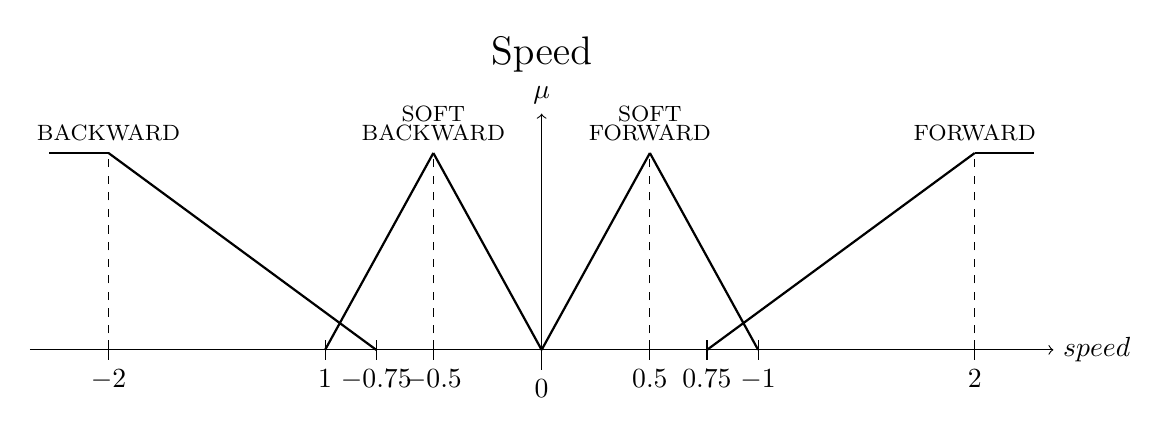
\begin{tikzpicture}
		\draw [->](6,-0.25)--(6,3) node[anchor = south]
			{$\mu$};
		\draw [->](-0.5,0)--(12.5,0) node[right]{$speed$};
		\node[anchor = north] at (6,-0.25) {$0$};
		
		\node at (6,3.75) {\Large Speed};
		\node at (0.5,2.75) {\footnotesize BACKWARD};
		
		\node at (4.625,3) {\footnotesize SOFT};
		\node at (4.625,2.75) {\footnotesize BACKWARD};
		
		\node at (11.5,2.75) {\footnotesize FORWARD};
		
		\node at (7.375,3) {\footnotesize SOFT};
		\node at (7.375,2.75) {\footnotesize FORWARD};	
		
		\draw (0.5,0.125) -- (0.5,-0.125) 
			node[anchor = north] {$-2$};
		\draw[dashed] (0.5,0) -- (0.5,2.5); 
			
		\draw (11.5,0.125) -- (11.5,-0.125)
			node[anchor = north] {$2$};
		\draw[dashed] (11.5,0) -- (11.5,2.5);				
		
		\draw (8.75,0.125) -- (8.75,-0.125)
			node[anchor = north] {$-1$};
			
		\draw (3.25,0.125) -- (3.25,-0.125)
			node[anchor = north] {$1$};	
		
		\draw (3.9,0.125) -- (3.9,-0.125)
			node[anchor = north] {$-0.75$};
			
		\draw (8.1,0.125) -- (8.1,-0.125)
			node[anchor = north] {$0.75$};		
		
		\draw (4.625,0.125) -- (4.625,-0.125)
			node[anchor = north] {$-0.5$};
		\draw[dashed] (4.625,0) -- (4.625,2.5);
			
		\draw (7.375,0.125) -- (7.375,-0.125)
			node[anchor = north] {$0.5$};		
		\draw[dashed] (7.375,0) -- (7.375,2.5);	
		
		\draw[thick] (-0.25,2.5) -- (0.5,2.5);
		\draw[thick] (11.5,2.5) -- (12.25,2.5);
		
		\draw[thick] (0.5,2.5) -- (3.9,0);
		\draw[thick] (11.5,2.5) -- (8.1,0);
		
		\draw[thick] (8.75,0) -- (7.375,2.5);
		\draw[thick] (7.375,2.5) -- (6,0);		
		
		\draw[thick] (3.25,0) -- (4.625,2.5);
		\draw[thick] (4.625,2.5) -- (6,0);		
	\end{tikzpicture}
\end{document}